\subsection{Prototype model}
Ud fra vores vision om et receptfornyelsesmodul og vores MoSCoW prioriteringer, har vi udviklet nedenstående ER-diagram over vores domæne:
\\
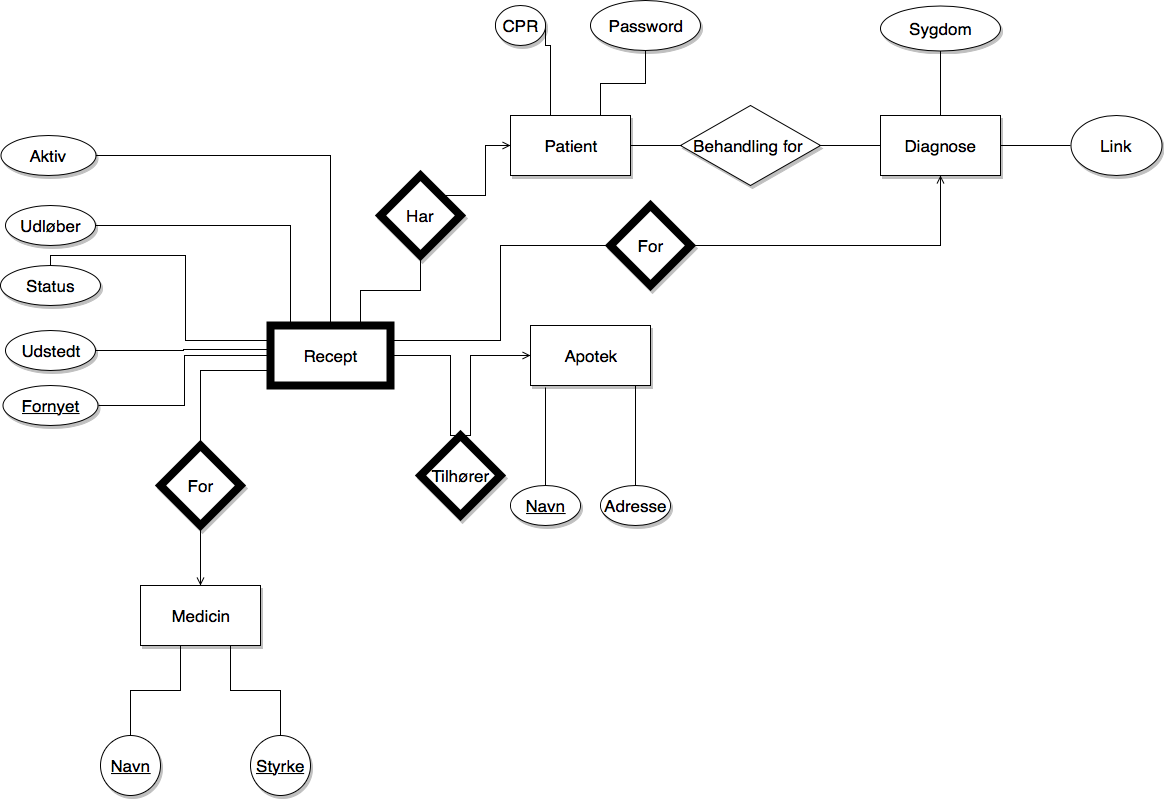
\includegraphics[width=\linewidth]{Materials/Prototype/ER_prototype}\\
Vores 'recept' entitet kan unikt identificeres ud fra vores andre entiteters nøgler, og er derfor lavet til en weak entity. 'Aptotek' entitetens navne-attribut er ikke lavet til en nøgle, da dette ville tillade at fornye den samme recept flere gange blot ved at ændre, hvor man ønsker at afhente medicinen.\\
Blandt vores ønskede funktioner er historik og medicinkort. For at implementere en historik-funktion, har det været nødvendigt at tilføje en 'Aktiv' attribut til 'recept' entiteten for at skelne mellem tidligere og nuværende recepter. Ved at lave en query på alle recepter, som tilhører et specifikt CPR-nummer, kan vi finde brugerens historik, mens at vi ved at lave en query på et CPR-nummer og angive 'Aktiv' attributten som sand, finder vi de aktive recepter for patienten.\\
Medicinkortet kan ligeledes konstrueres ud fra 'recept' entiteten samt hvilken patient, som ønsker at se sit medicinkort.\\ 
Det har derfor ikke været nødvendigt at lave entiteter til disse features.\\

Vi har herefter omsat vores entiteter til tabeller på samme vis som beskrevet i \textit{'Database Systems. The Complete Book'}\footnote{Prentice Hall, Database Systems. The Complete Book, s. 157-163}. Mange af vores entiteter kan laves direkte til tabeller, som ses nedenfor:
\begin{align*}
	&\textrm{Patient}(\textrm{\underline{CPR}, Password})\\
	&\textrm{Apotek}(\textrm{\underline{Navn}, Addresse})\\
	&\textrm{Medicin}(\textrm{\underline{Navn}, \underline{Styrke}})\\
\end{align*}
Ligeledes kan 'Diagnose' laves direkte. Denne tabel vil komme til at indeholde alle de diagnoser, som kan gives, og er nødvendig, da en patient kan have mere end én diagnose. Et link til patienthåndbogen for hver diagnose gemmes også.
\begin{equation*}
\textrm{Diagnose}(\textrm{\underline{Sygdom}, Link})
\end{equation*}
Vi har herefter vores 'Recept' entitet. Denne er weak og henter nøgler fra de fleste andre entiteter. 'Status'-attributten vil blive benyttet i overensstemmelse med vores vision om, at patienten selv skal kunne følge med i receptfornyelsesprocessen. 'Udstedt'-attributten vil blive benyttet af medicinkortet og vil aldrig ændre sig, da den repræsenterer, hvornår patienter første gang blev ordineret med medicinen. 'Udløber'-attributten vil blive benyttet til at sende reminders til patienterne.
\begin{equation*}
	\textrm{Recept}(\textrm{\underline{MedNavn}, \underline{MedStyrke}, \underline{PatCPR}, \underline{fornyet}, ApoNavn, status, udstedt, udløber, aktiv})
\end{equation*}
Hvis vi skulle lave vores relationer om til tabeller, ville der blive en masse redundancy, da alle på nær en enkelt relation allerede vil være subsets af andre tabeller. Derfor er den eneste relation som bliver lavet om til en tabel 'Behandles for'. Her vil begge nøgler være foreign keys til henholdsvis 'Patient' og 'Diagnose'.
\begin{equation*}
\textrm{BehandlesFor}(\textrm{\underline{PatCPR}, \underline{Sygdom}})
\end{equation*}
For at normalisering giver mening, kræver det, at vores tabeller indholder functional dependencies. Den eneste tabel, som vi vurderer indeholder en functional dependency, er 'Recept', hvor attributten fornyet kan give udløber. Men vi vurderer, at hvis lægen selv indskriver en udløbsdato på recepterne, vil det give lægen mere fleksibilitet i systemet til at tilpasse behandlinger. Da udløbsdatoen fastsættes af lægen, er der ikke længere nogen functional dependency, og vi kan ikke udføre normalisering.
